\chapter{Dodatečná vylepšení}

Jedná se o vylepšení, která vznikla kvůli ostatním vylepšením, nebo jako rychlá zlepšení chování KernelSharku. Pro každé z nich bude stručně popsán návrh, řešení, použití a případná varování.

\section{Aktualizace kódu zaškrtávacích políček}

Nejpřímějším zlepšením byla aktualizace grafického kódu, aby využíval novější Qt API pro zaškrtávací políčka. V nové API se nahrazuje funkce QCheckBox::stateChanged za QCheckBox::checkStateChanged. Hlavní změna se týká v argumentu značící zaškrtnutí - předtím stačilo dodat argument typu int, od Qt 6.7 ale nová funkce vyžaduje jednu z enumerovaných možností specifických pro QCheckBox.

Aktualizace nakonec spočívala pouze v nahrazení signálu stateChanged na checkStateChanged a použití výčtových hodnot (dle původního čísla) namísto pouze celých čísel.

KernelShark původně vynucoval v sestavení Qt verze 6.3, nyní vyžaduje alespoň verzi 6.7, aby mohl využít novější signál pro zaškrtávací políčka.

Změněné soubory: nejvyšší \emph{CMakeLists.txt} KernelSharku (v KS\_fork adresáři), \emph{KsTraceViewer.hpp/cpp}, \emph{KsCaptureDialog.hpp/cpp}, \emph{KsMainWindow.hpp/cpp}. Značkou modifikace v C++ kódu a CMake instrukcích je UPDATE CBOX STATES.

Pokud mají v plánu vývojáři KernelSharku či jeho pluginů dále pracovat s KernelSharkem, musejí tedy použít alespoň Qt6 verze 6.7.0.

\section{Zpřístupnění barev užívaných v grafu}

Modifikace je pouze zpřístupnění barevných tabulek, které KernelShark používá pro streamy, CPU a procesy. Díky zpřístupnění pak mohou tyto tabulky využívat i jiné části programu, nebo i pluginy. Jedná se o pouhé získání const reference na objekty využívané uvnitř KsGLWidget objektu. Přirozeně se jedná o malé úpravy, lokalizované v souboru \emph{KsGLWidget.hpp}, se kódovou značkou GET COLORS. K využití této modifikace stačí mít přístup k GL objektu a zavolat nové metody.

K využití přes pluginy se váže varování - pokud si KernelShark uloží do relace plugin, který využívá tuto modifikaci, ale načtení pluginu není dokonalé, program při první snaze o získání hodnoty z jakékoliv z tabulek spadne. Plugin je nedokonale načten vždy, pokud KernelShark načte relaci s daným pluginem, ale ten není předem explicitně načten uživatelem, tedy skrze argumenty při spouštění, nebo přes GUI. Další možnou podmínkou je, že plugin není postaven jako oficiální pluginy KernelSharku, tedy během sestavování KernelSharku samotného. Takto lze postavit například plugin Stacklook. Tato podmínka ovšem nebyla rigorózně otestována a je to spíše pouhá domněnka. Chybě se lze vyhnout třemi způsoby: buď uživatel vždy explicitně načte plugin, nebo plugin nebude tyto tabulky využívat, nebo bude obsahovat výchozí hodnotu, kterou použije namísto tabulek při načtení z relace - barevné tabulky se využijí až později, například až pokud si je uživatel zapne v konfiguraci pluginu.

Tuto modifikaci využívají pluginy Stacklook a Naps pro barvy procesů, a modifikace NUMA Topology Views pro barvy procesorů.

Příklad: Stacklook nabízí možnost barvit tlačítka dle barev procesů, kterým patří, viz obrázek \ref{obr01:modif-get-colors}.

\begin{figure}[p]\centering
    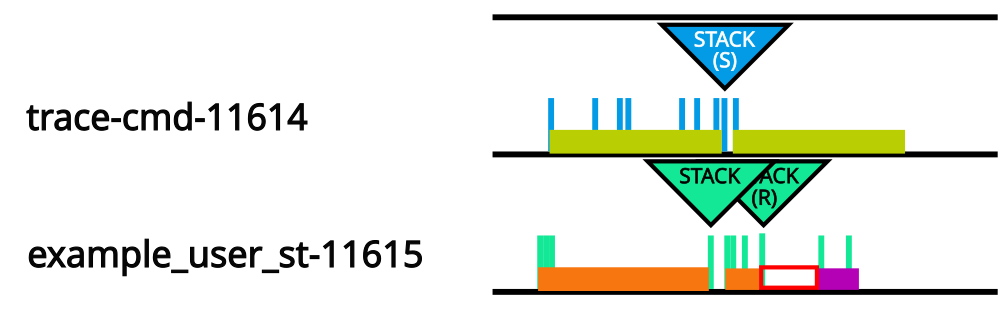
\includegraphics[width=140mm]{img/modif-get-colors-traced.png}
    \caption{Stacklook tlačítko využívá barvu, kterou KernelShark udělil procesu.}
    \label{obr01:modif-get-colors}
\end{figure}

\section{Reakce objektů v grafu na přejetí myší}

Tato modifikace dodala všem potomkům třídy KsPlot::PlotObject, jednodušeji plot-objekty, veřejnou metodu pro reakci na přejetí myší a redefinovatelnou privátní virtuální metodu, kterou veřejná metoda volá pro viditelný objekt. Privátní metoda má výchozí definici prázdnou. Krom toho je dodána detekce přejetí přes plot-objekt v grafu a reakce na přejetí. Toto chování bylo vsunuto na konec zpracování události pohybu myši a funguje podobně jako detekce dvojitého kliknutí. Soubory s modifikací: \emph{KsPlotTools.hpp} s novými metodami a \emph{KsGLWidget.cpp} pro vsunutou detekci a reakci. Kódová značka modifikace je MOUSE HOVER PLOT OBJECTS.

Nabízí se zde otázka, zdali je toto dostatečně výkonná implementace - myš se pohybuje často, objektů může být mnoho. Řešení musí vždy projít všechny plot-objekty a u každého se rozhodnout, zdali reagovat na myš či nikoliv. Při praktickém použití s rozumnými limity pro zobrazované plot-objekty (nedává smysl neustále zobrazovat tlačítka Stacklooku nad každým prvkem grafu, vedlo by to k přemíře informací) nenastaly problémy a nejvíc program zpomaloval objem dat a náhlé vykreslování objektů, nikoliv práce této modifikace. Pokud bude ale objektů příliš mnoho, výkon může být ovlivněn. Proto se optimalizace výkonu nechává jako \emph{rozšíření} této práce. Inspirací může být nahrazení lineárního prohledávání for-cyklem vyhledáváním přes souřadnice, tedy přes nějaké mapování souřadnic na objekty na těchto souřadnicích.

Tuto modifikaci používá hlavně plugin Stacklook.

\section{Měnitelné nápisy v hlavičce grafu}

Tato modifikace přidává do souborů \emph{KsTraceGraph.hpp/cpp} veřejnou funkci, s níž lze přepsat obsah informačního řádku KernelSharku. Jedná se o funkci typu setter, pouze nastaví hodnoty nápisů v informačním řádku.

K použití stačí mít k dispozici KsTraceGraph objekt. Pak se dá s modifikací pracovat i v pluginech a jiných částech KernelSharku.

V kódu lze tuto modifikaci nalézt pod značkou PREVIEW LABELS CHANGEABLE.

I zde se objevuje bug ze sekce o zpřístupnění barev využívaných v grafu, jenom se tentokrát netýká tabulek, nýbrž informačního řádku. Zde ale nelze spoléhat na nějaké výchozí hodnoty, tedy uživatel musí buď plugin vždy explicitně načíst, nebo nepoužívat plugin využívající tuto modifikaci.

Příklad použití: tlačítka Stacklooku (v červeném kroužku) žádají na přejetí myší o zobrazení několika prvků zásobníku kernelu, viz obrázek \ref{obr02:modif-preview-labels-changeable}.

\begin{figure}[p]\centering
    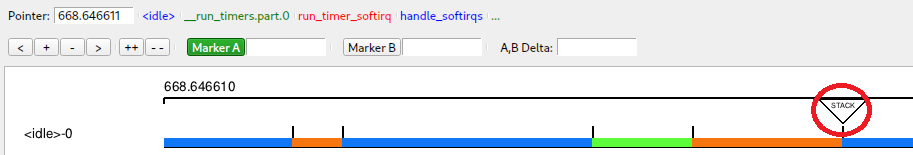
\includegraphics[width=140mm]{img/modif-preview-labels-changeable.png}
    \caption{Při přejetí kurzorem myši se vlevo nahoře informační řádek změní.}
    \label{obr02:modif-preview-labels-changeable}
\end{figure}

\section{NoBoxes}

Během vývoje se ukázalo, že některé záznamy by se neměly účastnit kreslení obdélníčků mezi záznamy (přesněji, mezi biny). Těmito záznamy jsou ty pro události od Couplebreaku a pro ftrace/kernel\_stack událost. Záznamy od Couplebreaku nezaznamenávají opravdovou práci. Události se zásobníkem dělají nepořádek hlavně po událostech typu sched/sched\_switch, po které by žádný obdélníček neměl být nakreslen, jelikož se přepnul CPU kontext. Jenže událost se zásobníkem je dle KernelSharku validní práce a tak se kreslí další obdélník.

Příklad špatného zobrazování je na obrázku \ref{obr03:modif-noboxes-bad}. Na tomto obrázku je ftrace/kernel\_stack událost vyznačená velkou svislou čarou vpravo, couplebreak/sched\_waking[target] je událost s velkou svislou čarou vlevo. Událost ftrace/kernel\_stack vytváří velký obdélník až do konce grafu, ačkoliv se událo po přepnutí kontextu a procesor ve skutečnosti po zachycení dále nepracuje. Událost couplebreak/sched\_waking[target], ačkoli neprovádí žádnou skutečnou práci na procesoru, vytváří dojem, že ano právě díky nakreslenému obdélníčku. V grafu CPU 1 je také velký obdélník, který začíná u události zachycení zásobníku kernelu a neměl by tedy být kreslen. Události zachycení zásobníku jsou časté a v grafu je více obdélníku spojených právě s nimi.

\begin{figure}[p]\centering
    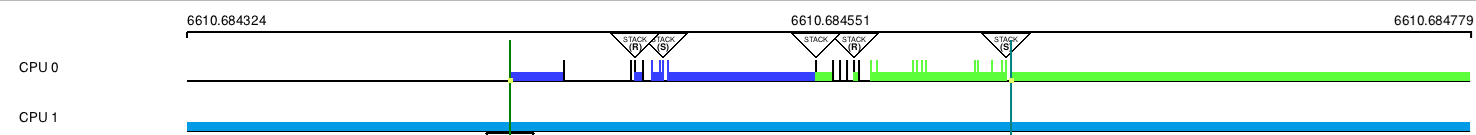
\includegraphics[width=140mm]{img/modif-noboxes-bad}
    \caption{Ne všechny obdélníky mezi záznamy by se měly vykreslovat, některé tvoří iluzi opravdové práce.}
    \label{obr03:modif-noboxes-bad}
\end{figure}

Toto chování je nepříjemné a tak byla snaha jej opravit. Nicméně KernelShark vykreslování obdélníčků řeší pro každé vykreslení zvlášť a pouze podle vlastností binů, tedy sdružení jednoho či více záznamů. V binech se pak lze spolehnout na málo, ale nejlépe na data viditelnosti, ve kterých mohou být nastaveny některé bity jako přepínače chování. Viditelnost binu lze ovlivnit viditelností záznamů, které sdružuje. Tak byla představena nová maska pro nastavování sedmého bitu pole viditelnosti pro záznamy, KS\_PLUGIN\_UNTOUCHED\_MASK. Tato maska značí, zdali se záznam účastní kreslení mezi-záznamových obdélníčků. Pokud bin využije viditelnost záznamu, který má daný bit nastaven na 0, bude moci toto nastavení detekovat. Při vykreslování obdélníčků pak žádné obdélníčky nezačínají a nekončí u binů s tímto bitem vynulovaným.

Maska byla přidána do enumerace pro masky viditelnosti. Tento výčet již předtím počítal s nějakým rozšířením, tak bylo jedno z volných bitových míst zabráno naší novou maskou. Rozšíření počítalo s nějakou KS\_X\_VIEW\_FILTER\_MASK pro volná místa - nicméně naše maska je spíše podobná masce KS\_PLUGIN\_UNTOUCHED\_MASK.

Na výběr záznamů, kterým se nastaví bit na 0, byl vytvořen plugin pro tuto modifikaci, nese název NoBoxes. V jeho kódu jsou zapsány události, na jejichž záznamy má být maska použita, plugin pak lze zapínat a vypínat jako každý jiný. Pokud plugin není načten, modifikace nemá na chod KernelSharku vliv.

Příklad fungujícího vylepšení je na obrázku \ref{obr04:modif-noboxes-good}. Oproti minulému obrázku (obrázek \ref{obr03:modif-noboxes-bad}) ubylo několik obdélníků a graf nyní odpovídá skutečné práci.

\begin{figure}[p]\centering
    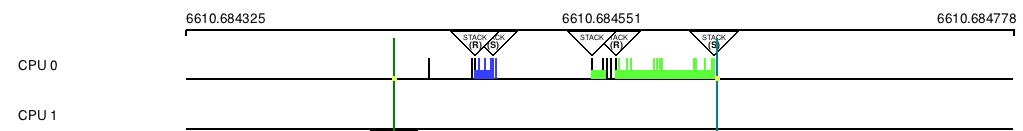
\includegraphics[width=140mm]{img/modif-noboxes-good}
    \caption{Vylepšení donutí některé obdélníky k tomu, aby nebyli nakresleny.}
    \label{obr04:modif-noboxes-good}
\end{figure}

Problém tohoto vylepšení je ale právě vykreslování obdélníků. Vykreslování se děje často a použitá implementace tohoto vylepšení při grafických změnách v hlavním okně KernelSharku často i přes vytvořené filtrování obdélník vykreslí. Při častých změnách pak nastává problikávání obdélníků, ačkoliv by vůbec kresleny být neměly. Oprava byla označena za rozšíření, jelikož objem práce k tomuto dodatku byl odhadnut na příliš velký.